\documentclass[11pt,letterpaper]{article}

\usepackage[utf8]{inputenc}
\usepackage[T1]{fontenc}
\usepackage[spanish,es-nodecimaldot,es-tabla]{babel}
\usepackage{lmodern}
\usepackage[margin=2.5cm]{geometry}
\usepackage{graphicx}
\usepackage{booktabs}
\usepackage{tabularx}
\usepackage{array}
\usepackage{xcolor}
\usepackage{caption}
\usepackage{enumitem}
\usepackage{listings}
\usepackage[hidelinks]{hyperref}

\definecolor{TecBlue}{RGB}{0,57,166}
\graphicspath{{../figures/}{./}}
\captionsetup{font=small,labelfont=bf}
\setlist{itemsep=2pt,topsep=4pt}
\newcolumntype{L}{>{\raggedright\arraybackslash}X}

\lstset{
  language=Python, basicstyle=\ttfamily\footnotesize, columns=fullflexible,
  keywordstyle=\color{TecBlue}\bfseries, commentstyle=\color{gray}\itshape,
  stringstyle=\color{teal!70!black}, frame=single, rulecolor=\color{gray!40},
  breaklines=true, showstringspaces=false, xleftmargin=4pt, xrightmargin=4pt,
  literate={á}{{\'a}}1 {é}{{\'e}}1 {í}{{\'i}}1 {ó}{{\'o}}1 {ú}{{\'u}}1
           {Á}{{\'A}}1 {É}{{\'E}}1 {Í}{{\'I}}1 {Ó}{{\'O}}1 {Ú}{{\'U}}1
           {ñ}{{\~n}}1 {Ñ}{{\~N}}1 {−}{{-}}1 {≥}{{$\geq$}}1
}

\begin{document}

% ---------------------------------------------------------------- Portada
\begin{titlepage}
  \centering
  \IfFileExists{LOGOTEC.png}{\includegraphics[width=0.38\textwidth]{LOGOTEC.png}\par\vspace{1cm}}{\vspace*{2cm}}
  {\Large Tecnológico de Monterrey\par}
  {\large Campus Guadalajara\par}
  \vspace{2.2cm}
  {\color{TecBlue}\Huge\bfseries Monitoreo de Saldo de Inventarios\par}
  \vspace{0.4cm}
  {\Large FEMSA Salud Chile (FCV)\par}
  \vspace{0.8cm}
  {\large Entregable 1: Primer avance --- automatización de alertas\par}
  \vspace{2cm}
  {\large\bfseries Integrantes:\par}
  \vspace{0.3cm}
  {\large
  Rafael Santamaría Heredia | A01646667\par
  Grethel Hernández Olivares | A01640912\par
  Matías Alfredo Hidalgo Guzmán | A01641323\par
  Daniel Rodríguez Peralta | A01646867\par}
  \vspace{1.2cm}
  {\large\bfseries Profesor:\par}
  {\large [Nombre del profesor] --- MA2004B (Gpo [X])\par}
  \vfill
  {\large [Fecha de entrega] de noviembre de 2026\par}
\end{titlepage}

\tableofcontents
\newpage

% ---------------------------------------------------------------- Introducción
\section{Introducción}

\subsection{Contexto}

El área de Auditoría Interna de FEMSA, dentro de la vertical financiera de la División Salud, revisa cada mes que el valor del inventario registrado en contabilidad corresponda con el inventario físico que reporta el sistema operativo. En la cadena de farmacias de Chile (FCV) esta revisión se apoya en dos reportes: el \emph{Kardex}, que detalla el stock y el costo de cada producto (SKU) al cierre del mes, y la \emph{balanza de comprobación}, que contiene el saldo contable de la cuenta de existencias.

Actualmente el proceso es manual. Se descargan ambos reportes, se concilian en Excel, se calcula la antigüedad de las partidas y se revisa una muestra de ellas. El riesgo que se busca controlar es la \textbf{sobrevaluación de inventarios} (control IN-SF045, conciliación): que los estados financieros reporten un inventario mayor al que realmente existe, ya sea por diferencias entre el módulo operativo y la contabilidad o por mercancía que, por su antigüedad, ya no tiene el valor con el que está registrada. En una farmacia este segundo punto es especialmente relevante, porque buena parte del inventario tiene fecha de caducidad.

Para el reto, el área compartió siete meses de información (enero a julio de 2026) y un archivo de Excel con su propuesta de alertas para julio, que incluye las fórmulas con las que hoy construyen las variables y un tablero resumen.

\subsection{Objetivos}

El objetivo general del proyecto es pasar de una revisión manual por muestreo a un esquema de auditoría continua sobre el 100\% de las partidas, con reglas de negocio automatizadas, un tablero interactivo y un componente predictivo basado en cadenas de Markov.

Para este primer avance los objetivos específicos son:
\begin{enumerate}
  \item Explorar y documentar las fuentes de datos (Kardex y balanza), incluyendo los problemas de calidad que presentan.
  \item Traducir a código modular de Python las fórmulas que el equipo de FEMSA usa en Excel para construir las variables de alerta.
  \item Demostrar que el código reproduce los resultados del archivo de ejemplo.
  \item Integrar Kardex y balanza para obtener la tabla de trabajo de un mes (enero) y dejar el proceso listo para cualquier otro mes.
\end{enumerate}

\subsection{Justificación}

La conciliación entre el Kardex y la contabilidad involucra más de 15 mil partidas por mes. Revisarlas a mano obliga a trabajar con muestras y depende de hojas de cálculo con fórmulas que se copian de un mes a otro, lo que facilita errores difíciles de detectar. Durante la exploración encontramos ejemplos concretos de esto: valores de antigüedad que no corresponden con su propia fórmula, una columna de control con un valor fijo en lugar de una regla y renglones de subtotales mezclados con el detalle.

Automatizar las reglas permite revisar todas las partidas cada mes con el mismo criterio, dejar trazabilidad de cada resultado y liberar tiempo del auditor para analizar las excepciones en lugar de construir la conciliación. Además, contar con una tabla mensual consistente es el requisito para la siguiente etapa del proyecto: estimar, mediante cadenas de Markov, qué proporción del inventario que hoy está en buen estado pasará a estar estancado en los próximos meses.

% ---------------------------------------------------------------- Datos
\section{Descripción de los datos}

\subsection{Contexto de los datos}

Se recibieron 16 archivos de Excel. Los nombres de productos y cuentas vienen anonimizados (\texttt{SKU\_000001}, \texttt{CTA\_000184}) y los importes están en pesos chilenos (CLP).

\begin{table}[h]
\centering\small
\begin{tabularx}{\textwidth}{@{}l c L@{}}
\toprule
Archivo & Cantidad & Contenido \\
\midrule
\texttt{INV\_Kardex\_AAAAMM.xlsx} & 7 & Detalle del inventario por SKU al cierre de cada mes (hoja \texttt{DETALLE KARDEX}) y una tabla dinámica con el valor por semáforo y el recetario (\texttt{TD DETA}). \\
\texttt{AAAAMM\_Balanza.xlsx} & 7 & Balanza de comprobación de 8 columnas de FCV, con unas 850 cuentas. \\
Propuesta de alertas & 1 & Archivo de ejemplo del área para julio: Kardex con fórmulas, tablero, criterios y detalle de alertas. \\
\texttt{Consulta\_TC.xlsx} & 1 & Tipo de cambio CLP a MXN de Banco de México (no se usa en este avance). \\
\bottomrule
\end{tabularx}
\caption{Archivos recibidos.}
\end{table}

La cuenta 111080001 (existencias) que menciona el planteamiento aparece en las balanzas como \texttt{CTA\_000184 EXISTENCIAS}. El inventario contable incluye además un componente de \emph{recetario} (entre 476 y 521 millones CLP al mes) que no está en el detalle por SKU; su valor solo aparece en la tabla dinámica \texttt{TD DETA}.

\subsection{Estructura}

\begin{table}[h]
\centering\small
\begin{tabularx}{\textwidth}{@{}l l l L@{}}
\toprule
Variable & Tipo & Unidad & Significado \\
\midrule
\multicolumn{4}{@{}l}{\emph{Kardex (una fila por SKU y mes)}} \\
\texttt{PERIODO} & fecha & mes & Primer día del mes reportado. \\
\texttt{CODIGO} & texto & --- & Identificador del producto (SKU). \\
\texttt{STOCK} & entero & unidades & Existencia al cierre. \\
\texttt{COSTO} & real & CLP/unidad & Costo unitario. \\
\texttt{VALORIZACION} & real & CLP & Stock $\times$ costo. \\
\texttt{FULCOM} & fecha & --- & Fecha de la última compra; base para la antigüedad. \\
\texttt{UNID CONV} & real & --- & Unidad de conversión; se espera 1. \\
\texttt{LINEA}, \texttt{NOMBRE LINEA} & categórica & --- & Línea de negocio (8 líneas). \\
\texttt{POLITICA CJE} & categórica & --- & P1: el producto tiene canje con el proveedor; P0: no. \\
\midrule
\multicolumn{4}{@{}l}{\emph{Balanza (una fila por cuenta)}} \\
\texttt{Cuenta}, \texttt{Descripción} & texto & --- & Identificador y nombre de la cuenta. \\
Balance débito / crédito & real & CLP & Saldo deudor y acreedor; el saldo es su diferencia. \\
Movimiento del mes & real & CLP & Columna que usa el tablero de la propuesta. \\
\bottomrule
\end{tabularx}
\caption{Variables principales.}
\end{table}

El Kardex trae, además, columnas calculadas con fórmulas (antigüedad en meses, semáforo, alertas de stock, costo, conversión y duplicados, y un estado general). Estas son las que se reconstruyen en código (sección~\ref{sec:variables}).

\subsection{Calidad de los datos}

\begin{itemize}
  \item \textbf{Fechas de última compra posteriores al cierre.} Entre 68\% y 73\% de las partidas de cada mes (entre 10,444 y 11,166) tienen una \texttt{FULCOM} posterior al último día del periodo; representan cerca del 98\% del valor del inventario. En el Kardex de enero, por ejemplo, hay fechas hasta el 24 de mayo de 2026. La fórmula de antigüedad las lleva a 0 meses, por lo que quedan en verde. Es el hallazgo más importante, porque afecta directamente al semáforo y al modelo de Markov; una posible causa es un desplazamiento de fechas al anonimizar, y se consultará con el equipo de FEMSA.
  \item \textbf{Valores de antigüedad desactualizados.} En los Kardex mensuales, los valores guardados de \texttt{MESES ANTIG.} no corresponden con lo que da su propia fórmula: en julio solo coinciden en 65\% de las partidas. Por eso la antigüedad siempre se recalcula a partir de \texttt{FULCOM}.
  \item \textbf{Renglones de subtotales.} El Kardex de julio tiene cuatro renglones sin código al final del detalle, con totales de Kardex y GL que suman unos 234 mil millones CLP. Si no se excluyen, el inventario del mes casi se triplica.
  \item \textbf{Unidad de conversión.} Entre 107 y 117 partidas por mes tienen \texttt{UNID CONV} distinta de 1, y en abril, junio y julio hay dos partidas con \texttt{\#N/A}.
  \item \textbf{Columna de movimiento vacía.} En las balanzas de febrero a junio la columna \emph{Movimiento del mes} viene vacía; el saldo se toma de Balance débito $-$ crédito, que coincide con ella en enero y julio.
  \item \textbf{Controles fijos o circulares.} La alerta de duplicados es un texto fijo (``OK''), y la diferencia de valorización compara \texttt{VALORIZACION} con \texttt{STOCK}$\times$\texttt{COSTO}, cuando la primera se calcula precisamente así; por diseño siempre da cero.
  \item \textbf{Sin faltantes en campos clave.} No hay códigos duplicados (una vez quitados los subtotales), stocks negativos o en cero (salvo dos partidas en febrero), costos no positivos ni fechas vacías.
  \item \textbf{Política de semáforo.} Hay tres definiciones: el planteamiento del reto (0--30 días y más de un año), la hoja de criterios de la propuesta (0--90, 91--180 y más de 180 días) y las fórmulas del Kardex (hasta 6, de 7 a 12 y más de 12 meses). Para replicar la propuesta se usa la última, dejando los límites como parámetros.
\end{itemize}

\subsection{Resumen estadístico}

La Tabla~\ref{tab:desc} resume las variables numéricas del Kardex de enero (15,272 partidas). Todas tienen una fuerte asimetría a la derecha: la media de la valorización es casi cuatro veces la mediana y unos pocos productos concentran valores muy altos. La antigüedad tiene mediana cero, reflejo de las fechas posteriores al cierre descritas arriba.

\begin{table}[h]
\centering\small
\begin{tabular}{@{}lrrrrrr@{}}
\toprule
Variable & Media & Mediana & Desv. est. & Mínimo & Q3 & Máximo \\
\midrule
Stock (unidades) & 1,288.2 & 503 & 5,460.8 & 1 & 1,437 & 292,264 \\
Costo (CLP) & 11,806.3 & 4,460.8 & 77,053.0 & 0.04 & 10,130.4 & 4,785,281.1 \\
Valorización (miles CLP) & 7,751.3 & 2,109.3 & 21,943.6 & 0.0 & 9,372.2 & 1,669,108.0 \\
Antigüedad (meses) & 7.7 & 0 & 23.2 & 0 & 1 & 166 \\
\bottomrule
\end{tabular}
\caption{Estadística descriptiva del Kardex, enero de 2026.}
\label{tab:desc}
\end{table}

Por línea de negocio (Tabla~\ref{tab:linea} y Figura~\ref{fig:linea}), Farmacia concentra el 55\% del valor y Belleza el 24\%. Mercaderías Varias es la línea de menor valor, pero la más envejecida: su mediana de antigüedad es de 45 meses y 269 de sus 395 partidas están en rojo. Por política de canje, las partidas sin canje (P0) tienen 1,484 partidas en rojo contra 656 de las que sí tienen (P1), lo que coincide con la prioridad que la propuesta da a las partidas P0 envejecidas.

\begin{table}[h]
\centering\small
\begin{tabular}{@{}lrrrr@{}}
\toprule
Línea & Partidas & Valor (millones CLP) & \% del valor & Partidas en rojo \\
\midrule
Farmacia & 4,671 & 65,338.9 & 55.2 & 271 \\
Belleza & 5,949 & 28,510.2 & 24.1 & 891 \\
Cuidado e higiene personal & 2,723 & 13,668.5 & 11.6 & 406 \\
Alimentos & 575 & 5,286.7 & 4.5 & 45 \\
Cuidado del bebé & 577 & 2,850.7 & 2.4 & 186 \\
Veterinaria & 216 & 1,514.9 & 1.3 & 52 \\
Distribuibles & 166 & 918.3 & 0.8 & 20 \\
Mercaderías varias & 395 & 289.8 & 0.2 & 269 \\
\bottomrule
\end{tabular}
\caption{Inventario por línea de negocio, enero de 2026.}
\label{tab:linea}
\end{table}

\begin{figure}[h]
\centering
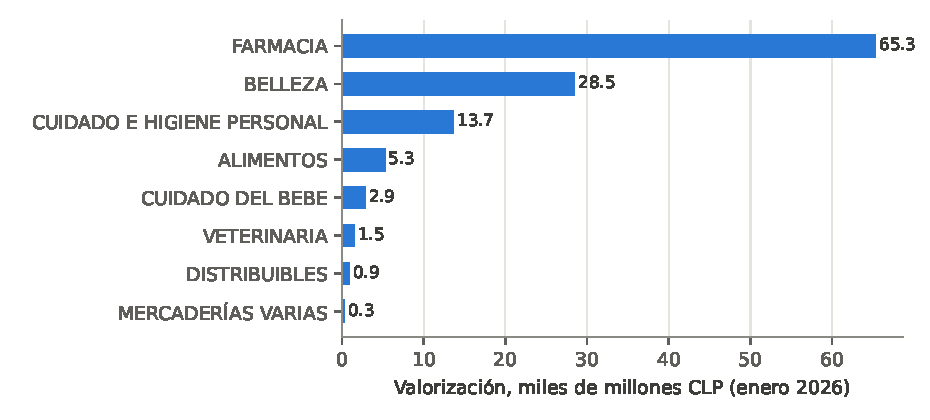
\includegraphics[width=0.85\textwidth]{valor_por_linea_enero.pdf}
\caption{Valorización por línea de negocio, enero de 2026.}
\label{fig:linea}
\end{figure}

A lo largo de los siete meses (Figura~\ref{fig:saldo}), el saldo contable de existencias se movió entre 114 y 128 mil millones CLP. El único cambio mensual igual o mayor a 5\% fue el de mayo ($-7.35\%$). El número de partidas en rojo se mantuvo entre 1,900 y 2,150, mientras que las partidas en ámbar casi se duplicaron en junio (Figura~\ref{fig:semaforo}).

\begin{figure}[h]
\centering
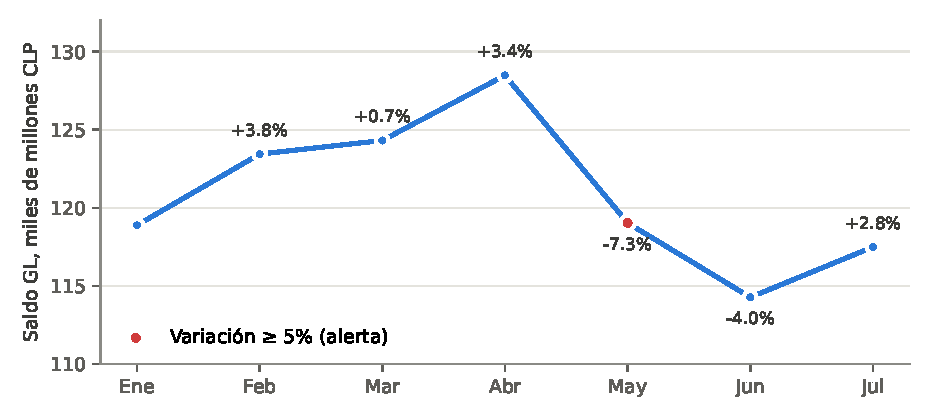
\includegraphics[width=0.85\textwidth]{saldo_gl_mensual.pdf}
\caption{Saldo contable de la cuenta de existencias y variación respecto al mes anterior.}
\label{fig:saldo}
\end{figure}

\begin{figure}[h]
\centering
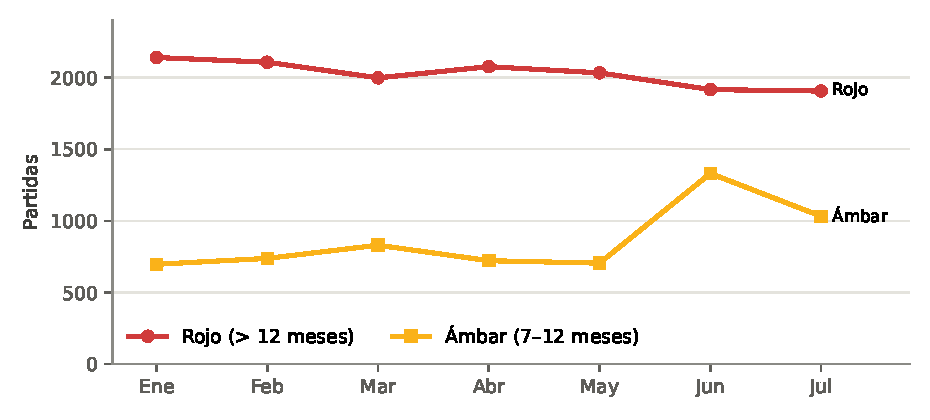
\includegraphics[width=0.85\textwidth]{partidas_semaforo_mensual.pdf}
\caption{Partidas en rojo y ámbar por mes (criterio de la propuesta: más de 12 y de 7 a 12 meses).}
\label{fig:semaforo}
\end{figure}

% ---------------------------------------------------------------- Metodología
\clearpage
\section{Metodología}

\subsection{Procesamiento de datos}

El proceso de cada mes cruza tres fuentes:

\begin{enumerate}
  \item \textbf{Kardex.} Se lee la hoja \texttt{DETALLE KARDEX}, se descartan los renglones sin código y se conservan solo las columnas de entrada (periodo, código, stock, costo, fecha de última compra, unidad de conversión, línea y política). Las columnas calculadas del archivo se ignoran porque se reconstruyen.
  \item \textbf{Balanza.} Se lee la hoja \texttt{FCV} (saltando los siete renglones de encabezado) y se obtiene el saldo de \texttt{CTA\_000184} como Balance débito $-$ crédito.
  \item \textbf{Recetario.} Se toma de la tabla \texttt{TD DETA} del propio Kardex, en el renglón del periodo.
\end{enumerate}

Con esto se calculan las columnas de alerta por partida y, a nivel mes, la conciliación: el inventario conciliable (detalle del Kardex más recetario) se compara contra el saldo contable, con una tolerancia de 0.1\% del GL, igual que en el tablero de la propuesta. Al juntar varios meses se calcula la variación del saldo contra el mes anterior.

El proceso es reproducible: el código está versionado en GitHub, las dependencias se fijan con \texttt{uv}, y los datos se encriptan con \texttt{age} y se versionan con DVC en DagsHub, de modo que cualquier integrante puede regenerar las tablas con los mismos archivos de entrada.

\subsection{Construcción de variables}
\label{sec:variables}

Cada fórmula del archivo de Excel se tradujo a una función en \texttt{src/alertas\_inventario.py} (Tabla~\ref{tab:formulas}). El script \texttt{src/construir\_columnas.py} aplica estas funciones a uno o varios meses y genera dos tablas en \texttt{data/processed/}: \texttt{kardex\_alertas.csv}, con el detalle por SKU y mes, y \texttt{resumen\_mensual.csv}, con una fila de indicadores por mes.

\begin{table}[h]
\centering\small
\begin{tabularx}{\textwidth}{@{}l L l@{}}
\toprule
Variable & Regla (fórmula de Excel) & Función \\
\midrule
Meses de antigüedad & Meses de calendario entre el cierre del periodo y \texttt{FULCOM}; mínimo 0 & \texttt{meses\_antiguedad} \\
Alerta de antigüedad & Sin fecha; rojo si $>12$; ámbar si $>6$; verde en otro caso & \texttt{alerta\_antiguedad} \\
Diferencia de valorización & Valorización $-$ stock $\times$ costo & \texttt{dif\_valorizacion} \\
Alerta de stock & Negativo si $<0$; cero si $=0$ & \texttt{alerta\_stock} \\
Alerta de costo & Inválido si $\le 0$ & \texttt{alerta\_costo} \\
Alerta de conversión & Inválida si vacía o $\le 0$; revisar si $\neq 1$ & \texttt{alerta\_conversion} \\
Alerta de duplicado & Código repetido en el mes & \texttt{alerta\_duplicado} \\
Estado general & Revisar si hay rojo o cualquier alerta; monitorear si ámbar & \texttt{estado\_general} \\
Conciliación & $|$(Kardex $+$ recetario) $-$ GL$| \le 0.1\%$ del GL & \texttt{conciliacion} \\
Variación mensual & $|\Delta$ saldo$| \ge 5\%$ respecto al mes anterior & \texttt{variacion\_mensual} \\
Naturaleza contraria & Valorización negativa o saldo acreedor en existencias & \texttt{naturaleza\_contraria} \\
\bottomrule
\end{tabularx}
\caption{Variables construidas y función que las calcula.}
\label{tab:formulas}
\end{table}

Como ejemplo, la antigüedad y el estado general quedan así:

\noindent\begin{minipage}{\linewidth}
\begin{lstlisting}
def meses_antiguedad(periodo, fulcom):
    # Excel: =IF(G2="","",MAX(0,(YEAR(EOMONTH(A2,0))-YEAR(G2))*12
    #                          +MONTH(EOMONTH(A2,0))-MONTH(G2)))
    cierre = periodo + pd.offsets.MonthEnd(0)
    meses = (cierre.dt.year - fulcom.dt.year) * 12 + (cierre.dt.month - fulcom.dt.month)
    return meses.clip(lower=0).astype("Int64")

def estado_general(df):
    revisar = ((df["ALERTA_ANTIG"] == "ROJO") | (df["ALERTA_STOCK"] != "OK")
               | (df["ALERTA_COSTO"] != "OK") | (df["DIF_VALORIZACION"].abs() > 1)
               | (df["ALERTA_CONVERSION"] != "OK") | (df["ALERTA_DUPLICADO"] != "OK"))
    monitorear = df["ALERTA_ANTIG"] == "ÁMBAR"
    return np.select([revisar, monitorear], ["REVISAR", "MONITOREAR"], default="OK")
\end{lstlisting}
\end{minipage}

Hay dos diferencias intencionales con el Excel. La alerta de duplicados se calcula en lugar de ser un valor fijo, como recomienda la propia propuesta. Y cuando la unidad de conversión trae \texttt{\#N/A}, Excel propaga el error y la partida queda sin estado; en el código se marca como inválida y pasa a revisión, para que no desaparezca del reporte.

\subsection{Validación contra el archivo de ejemplo}

El notebook \texttt{notebooks/02\_replica\_propuesta.ipynb} procesa julio con el código y lo compara contra la propuesta:

\begin{itemize}
  \item \textbf{Por partida:} las 15,357 partidas coinciden en todas las columnas calculadas, excepto las dos con \texttt{\#N/A} en la unidad de conversión, por la diferencia intencional descrita arriba.
  \item \textbf{Tablero:} coinciden el saldo GL (117,495,620,727 CLP), el inventario conciliable, la diferencia ($-0.37$ CLP), el estado ``conciliado'', los conteos y valores por color (por ejemplo, 1,906 partidas en rojo por 177.8 millones CLP), las alertas de conversión (109 partidas) y el top 10 de partidas rojas. Solo el total para revisar difiere en dos partidas (1,981 contra 1,979).
  \item \textbf{Detalle de alertas:} la lista de partidas a revisar o monitorear es la misma (3,005), más las dos partidas con \texttt{\#N/A}.
\end{itemize}

Con el proceso validado se construyó la tabla de enero (15,272 partidas y 21 columnas) y el resumen de los siete meses (Tabla~\ref{tab:mensual}). Todos los meses concilian dentro de la tolerancia; la mayor diferencia es la de abril, de 19.72 CLP. Con un umbral estricto de 0\%, como el del planteamiento, ningún mes cuadraría exactamente por diferencias de centavos, por lo que conviene acordar la tolerancia con el equipo de FEMSA.

\begin{table}[h]
\centering\small
\begin{tabular}{@{}lrrrrrrr@{}}
\toprule
Mes & GL (mill. CLP) & Recetario & Diferencia & Var. GL & Rojo & Ámbar & Revisar \\
\midrule
Ene & 118,886.7 & 508.6 & $-0.43$ & --- & 2,140 & 697 & 2,216 \\
Feb & 123,437.2 & 511.1 & 0.31 & $+3.8\%$ & 2,107 & 738 & 2,191 \\
Mar & 124,306.9 & 485.8 & 0.01 & $+0.7\%$ & 1,998 & 830 & 2,078 \\
Abr & 128,473.3 & 486.9 & 19.72 & $+3.4\%$ & 2,076 & 722 & 2,158 \\
May & 119,034.5 & 478.6 & 0.49 & $\mathbf{-7.3\%}$ & 2,033 & 705 & 2,111 \\
Jun & 114,277.3 & 476.0 & 0.29 & $-4.0\%$ & 1,916 & 1,331 & 1,991 \\
Jul & 117,495.6 & 520.5 & $-0.37$ & $+2.8\%$ & 1,906 & 1,032 & 1,981 \\
\bottomrule
\end{tabular}
\caption{Resumen mensual. El recetario está en millones CLP y la diferencia (Kardex $+$ recetario $-$ GL) en CLP. En negritas, la única variación que activa la alerta.}
\label{tab:mensual}
\end{table}

\subsection{Siguientes pasos}

\begin{itemize}
  \item Resolver con el equipo de FEMSA las fechas de última compra posteriores al cierre, la política de semáforo vigente y la tolerancia de conciliación.
  \item Construir el tablero en Power BI a partir de \texttt{kardex\_alertas.csv} y \texttt{resumen\_mensual.csv}.
  \item Estimar las matrices de transición entre rangos de antigüedad con los SKU que aparecen en meses consecutivos (13,788 están presentes en los siete), para proyectar la proporción del inventario que pasará a ámbar o rojo.
\end{itemize}

\end{document}
